% This is the Reed College LaTeX thesis template. Most of the work 
% for the document class was done by Sam Noble (SN), as well as this
% template. Later comments etc. by Ben Salzberg (BTS). Additional
% restructuring and APA support by Jess Youngberg (JY).
% Your comments and suggestions are more than welcome; please email
% them to cus@reed.edu
%
% See http://web.reed.edu/cis/help/latex.html for help. There are a 
% great bunch of help pages there, with notes on
% getting started, bibtex, etc. Go there and read it if you're not
% already familiar with LaTeX.
%
% Any line that starts with a percent symbol is a comment. 
% They won't show up in the document, and are useful for notes 
% to yourself and explaining commands. 
% Commenting also removes a line from the document; 
% very handy for troubleshooting problems. -BTS

% As far as I know, this follows the requirements laid out in 
% the 2002-2003 Senior Handbook. Ask a librarian to check the 
% document before binding. -SN

%%
%% Preamble
%%
% \documentclass{<something>} must begin each LaTeX document
\documentclass[12pt,twoside]{reedthesis}
% Packages are extensions to the basic LaTeX functions. Whatever you
% want to typeset, there is probably a package out there for it.
% Chemistry (chemtex), screenplays, you name it.
% Check out CTAN to see: http://www.ctan.org/
%%
\usepackage{graphicx,latexsym} 
\usepackage{amssymb,amsthm,amsmath}
\usepackage{longtable,booktabs,setspace} 
\usepackage{chemarr} %% Useful for one reaction arrow, useless if you're not a chem major
\usepackage[hyphens]{url}
\usepackage{rotating}
\usepackage{natbib}
\usepackage[english]{babel}
\usepackage{amsmath}
\usepackage{multirow}
% Comment out the natbib line above and uncomment the following two lines to use the new 
% biblatex-chicago style, for Chicago A. Also make some changes at the end where the 
% bibliography is included. 
%\usepackage{biblatex-chicago}
%\bibliography{thesis}

% \usepackage{times} % other fonts are available like times, bookman, charter, palatino

\title{On Forecasting Solar Flares via. the Bayesian Blocks Method using Flare Data from Terrestrial Solar Observatories vs. Extraterrestrial Detectors}
\author{Tenzin Sangpo}
% The month and year that you submit your FINAL draft TO THE LIBRARY (May or December)
\date{December 2019}
\division{Mathematics and Natural Sciences}
\advisor{Andrew P. Bray}
%If you have two advisors for some reason, you can use the following
%\altadvisor{Your Other Advisor}
%%% Remember to use the correct department!
\department{Mathematics}
% if you're writing a thesis in an interdisciplinary major,
% uncomment the line below and change the text as appropriate.
% check the Senior Handbook if unsure.
%\thedivisionof{The Established Interdisciplinary Committee for}
% if you want the approval page to say "Approved for the Committee",
% uncomment the next line
%\approvedforthe{Committee}

\setlength{\parskip}{0pt}
%%
%% End Preamble
%%
%% The fun begins:
\begin{document}

  \maketitle
  \frontmatter % this stuff will be roman-numbered
  \pagestyle{empty} % this removes page numbers from the frontmatter

% Acknowledgements (Acceptable American spelling) are optional
% So are Acknowledgments (proper English spelling)
    \chapter*{Acknowledgements}
	I want to thank a few people.

% The preface is optional
% To remove it, comment it out or delete it.
    \chapter*{Preface}
	This is an example of a thesis setup to use the reed thesis document class.
	
	

    \chapter*{List of Abbreviations}
		You can always change the way your abbreviations are formatted. Play around with it yourself, use tables, or come to CUS if you'd like to change the way it looks. You can also completely remove this chapter if you have no need for a list of abbreviations. Here is an example of what this could look like:

	\begin{table}[h]
	\centering % You could remove this to move table to the left
	\begin{tabular}{ll}
		\textbf{CME}  	&  Coronal Mass Ejection \\
		\textbf{SEP}  	&  Solar Energetic Particle \\
	\end{tabular}
	\end{table}
	

    \tableofcontents
% if you want a list of tables, optional
    \listoftables
% if you want a list of figures, also optional
    \listoffigures



% The abstract is not required if you're writing a creative thesis (but aren't they all?)
% If your abstract is longer than a page, there may be a formatting issue.
    \chapter*{Abstract}
    
	The Bayesian blocks approach to solar flare prediction relies not only on the optical classification of sunspots and the past flaring rate of a given cluster, but also the flaring record of an active region for events small and large. Studies implementing the refinement, however, run programs written in the Interactive Data Language (IDL), a proprietary programming language. This dissertation aims to employ the novel approach to forecast large flare occurrences via. Changepoint Analysis using the Pruned Exact Linear Time (PELT) algorithm in R, a more accessible platform. Available scientific literature on flares is discussed, the applied essentials in statistics, the theories of the respective methods are outlined, and simulations for the latter is presented to demonstrate how the method works in practice. Furthermore, forecasts from historical data acquired from terrestrial solar telescopes and the Geostationary Operational Environmental Satellites (GOES) under the National Oceanographic and Atmospheric Administration are compared with actual observations to ascertain both, the validity of the approach and the necessity of equipping satellites with flare detectors.             
	
	
	\chapter*{Dedication}
	You can have a dedication here if you wish.

  \mainmatter % here the regular arabic numbering starts
  \pagestyle{fancyplain} % turns page numbering back on

%The \introduction command is provided as a convenience.
%if you want special chapter formatting, you'll probably want to avoid using it altogether



    \chapter*{Introduction}
         \addcontentsline{toc}{chapter}{Introduction}
	\chaptermark{Introduction}
	\markboth{Introduction}{Introduction}
	% The three lines above are to make sure that the headers are right, that the intro gets included in the table of contents, and that it doesn't get numbered 1 so that chapter one is 1.

% Double spacing: if you want to double space, or one and a half 
% space, uncomment one of the following lines. You can go back to 
% single spacing with the \singlespacing command.
% \onehalfspacing
% \doublespacing
	
	Welcome to the \LaTeX\ thesis template. If you've never used \TeX\ or \LaTeX\ before, you'll have an initial learning period to go through, but the results of a nicely formatted thesis are worth it for more than the aesthetic benefit: markup like \LaTeX\ is more consistent than the output of a word processor, much less prone to corruption or crashing and the resulting file is smaller than a Word file. While you may have never had problems using Word in the past, your thesis is going to be about twice as large and complex as anything you've written before, taxing Word's capabilities. If you're still on the fence about  using \LaTeX, read the Introduction to LaTeX on the CUS site as well as skim the following template and give it a few weeks. Pretty soon all the markup gibberish will become second nature.

\section{Why use it?}
	
\LaTeX\ does a great job of formatting tables and paragraphs. Its line-breaking algorithm was the subject of a PhD.\thinspace thesis. It does a fine job of automatically inserting ligatures, and to top it all off it is the only way to typeset good-looking mathematics.

\section{Who should use it?}

Anyone who needs to use math, tables, a lot of figures, complex cross-references, IPA or who just cares about the final appearance of their document should use \LaTeX. At Reed, math majors are required to use it, most physics majors will want to use it, and many other science majors may want it also.


	
\chapter{On Solar Flares}
  
\section{Understanding Solar Flares}	
Solar flares are localized sudden and intense bursts of radiation from the sun that can last from several seconds to a few hours. Their concurrence with solar energetic particles (SEPs) and coronal mass ejections (CMEs), as well as their proximity to clusters of sunspots is well documented. In fact, the first solar flare was observed on September 1, 1805 by the astronomer Richard C. Carrington, and then later that year by Richard Hodgson, while monitoring sunspots. The flares manifested themselves in the middle of a sunspot group as two blotches of white-light rapidly brightening across the spectrum of visible electromagnetic (EM) radiation. They then dimmed as they moved before finally disappearing in a matter of minutes. But solar flares are more than mere flashes; they are tremendous explosions that occur on the surface of our resident star. The energy liberated from the said events can range from $10^{23}$ to $10^{25}$ joules. That is as much clout as a billion megatons of TNT which dwarfs the 50 million tons of TNT yield of ‘Tsar Bomba’, considered among the mightiest thermo-nuclear weapon ever conceived. Solar flares are the most powerful phenomenon in our solar system. \\

And the released energy manifests itself in various forms. Firstly, the materials encompassing the regions of interest can expect to be heated up to 20 million kelvins. The sun’s photosphere i.e. the outer shell from which light is emitted, sits at about 6,000 kelvins. Secondly, accelerated particles therein such as electrons, protons and ions can gain energy up to several giga electron-volts (GeV). And finally, there is strong plasma motion i.e. movement of said materials down a temperature or pressure gradient. The accelerated charged particles and heated matter motion in turn cause the emission of electromagnetic radiation across the entire electromagnetic spectrum i.e. radio, microwaves, visible light, ultraviolet, X-ray and gamma ray. \\

\section{Observing Solar Flares} 

The National Oceanographic and Atmospheric Administration (NOAA) oversees the satellites charged with detecting solar flares. The Geostationary Orbital Environmental Satellite – R Series (GOES-R) orbits the Earth on the geosynchronous orbit, about 22,236 miles above the ‘Blue Planet’, where it matches the revolution of the Earth about its axis. It is equipped with a Solar Ultraviolet Imager (SUVI) telescope and an X-ray spectrometer to constantly monitor the sun for flares. The telescope enables researchers to locate the flare on the sun while the spectrometer affords an estimate as to the magnitude of the flare strength. With this information, NOAA is able to determine if the explosion is well positioned and severe enough to approach Earth. The Deep Space Climate Observatory (DSCOVR) satellite positioned at a point of neutral gravity between the Earth and the sun can detect the approaching storm and issue space-weather warning about 15 to 60 minutes before it reaches Earth. Upon arrival, GOES-R can measure the magnetic fields as well as the radiation levels from the particles ejected from the sun at the geosynchronous orbit above the Earth due to this flare or explosion.\\

But solar telescopes around the globe have been making Hydrogen-alpha (H-alpha) spectral observations from Earth long before the first artificial satellite was even considered as a notion.  Hydrogen – the most abundant element in the Sun – can only exist in its atomic configuration in the sun’s outermost and visible regions where it is cool enough. The electron of a given hydrogen atom here can absorb energy and attain a higher energy level (n). But when the said electron drops to a lower energy level, it relinquishes the spare energy in the form of electromagnetic radiation. The emission in the visible spectrum occurs if electron falls to the energy level with n = 2 and is referred to as the Balmer Series. The H-alpha light specifically has a reddish hue and is emitted by hydrogen atoms when the electron falls from the energy level n = 3 to n = 2. Solar telescopes use H-alpha filters to isolate this light. Observatories may also capture images of the Sun at regular intervals to visually monitor and document solar flares. \\


\section{Classifying Solar Flares} 

Solar flares were previously classified on the basis of their H-alpha spectral observations in terms of brightness and size. For the former, a qualitative cataloguing of H-alpha intensity was employed with the designations to report flare brightness as shown in Table 1.1.  As for the latter, a measure of then emitting surface area in terms of \textit{Millionth of Solar Hemispherical Area} was considered to record flare size with the rubric shown in Table 1.2.\\

\begin{table}[h]
	\centering % You could remove this to move table to the left
	\begin{tabular}{lp{5cm}l}
		\hline
		\textbf{Category} &  \textbf{Non-abbreviated} \\
		\hline
		\textit{F}  		&  Faint \\
		\textit{N}  		&  Normal \\
		\textit{B}  		&  Bright \\
		\hline
	\end{tabular}
	\caption{H-alpha spectral observations in terms of flare brightness.}
	\end{table}

	
	
\begin{table}[h]
	\centering % You could remove this to move table to the left
	\begin{tabular}{lp{5cm}l}
		\hline
		\textbf{Category} &  \textbf{Size} \\ & (Millionths of Solar Hemispherical Area) \\
		\hline
		\textit{S}  		&  Less than 100 units \\
		\textit{1}  		&  Between 100 \& 250 units\\
		\textit{2}  		&  Between 250 \& 600 units \\
		\textit{3}  		&  Between 100 \& 1200 units \\
		\textit{4}  		&  More than 1200 units \\
		\hline
	\end{tabular}
	\caption{H-alpha spectral observations in terms of flare size.}
	\end{table}
	
	However, since solar flares also release their energy in the form of X-rays, they are also categorized on the basis of the brightness in their X-rays. The categorization of flares based on X-ray (100 - 800 pico-meters wavelength range) Peak Flux in \textit{Watts per Square-Meters} is as shown in Table 1.3.  \\

\begin{table}[h]
	\centering 
	\begin{tabular}{lp{5cm}l}
		\hline
		\textbf{Class} &  \textbf{Size} \\ & (Watts per Square-Meters) \\
		\hline
		\textit{A}  		&  Less  than  $10^{-7}$ units \\
		\textit{B}  		&  Between  $10^{-7}$ \& $10 ^{-6}$ units \\
		\textit{C}  		&  Between  $10^{-6}$ \& $10^{-5}$ units \\
		\textit{M}  		&  Between  $10^{-5}$ \& $10^{-4}$ units \\
		\textit{X}  		&  More  than  $10^{-4}$ units \\
		\hline
	\end{tabular}
	\caption{Flare classes on the basis of X-ray peak flux.}
	\end{table}
	
	
	The A-class flares are near background levels. Followed by B, C, M and X, each letter represents a 10-fold increase in energy output. So, an X is ten times an M and 100 times a C. Within each letter class there is a finer scale from 1 to 9. C-class and smaller flares are too weak to noticeably affect Earth. M-class flares can cause brief radio blackouts at the poles and minor radiation storms that might endanger astronauts. And then come the X-class flares. Although X is the last letter, there are flares more than 10 times the power of an X1, so X-class flares can go higher than 9. The most powerful flare measured with modern methods was in 2003, during the last solar maximum, and it was so powerful that it overloaded the sensors measuring it. The sensors cut out at X2.\\
	
	
	\begin{figure}[htbp] %  figure placement: here, top, bottom, or page
	   \centering
	   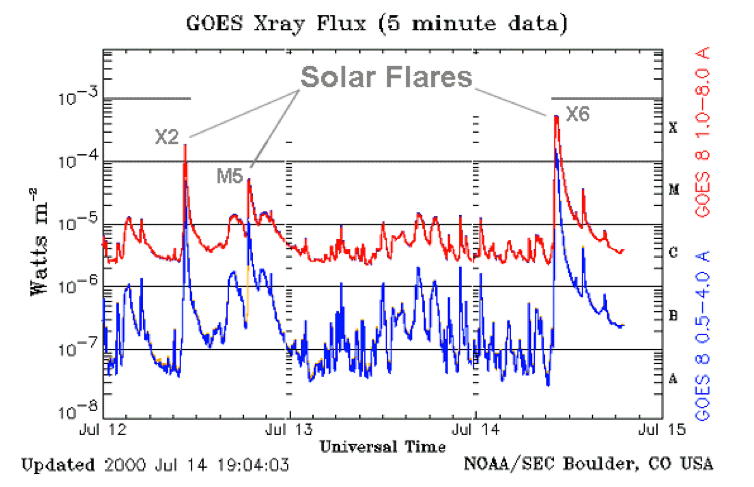
\includegraphics[width=4in]{osf1.png} 
	   \caption{Solar flares detected by NOAA satellites in July 2000}
	\end{figure}
	
	The measure of the latter – also called X-ray flux – is pivotal in characterizing the magnitude of the overall flare energy emitted. As was previously noted, GOES-R satellite orbiting the Earth are equipped with telescopes to locate the flares and with detectors to detect the X-rays in it. If the flare is severe enough to cause a geomagnetic storm, the DSCOVR satellite can issue a 15 to 60 minutes warning. \\
	
\section{How Flares Become} 

Like the Earth, the magnetic field of the sun is generated by the motion of electrically conducting fluids – plasma in case of the sun – within it. With the preponderance of evidence favoring the proximity of sunspots with solar flares, determining the structure of magnetic field around the former is pivotal to better comprehend and forecast the latter. It has been measurably observed that if and when the magnetic field is twisted or sheared, the otherwise separated field lines can cross over each other. The resulting short-circuiting causes a tremendous release of magnetic energy in the form of explosive flares. \\

This had been demonstrated by measurements on the orientation of magnetic field in active regions from the NASA-MSFC (Marshall Space Flight Center) Vector Magnetograph.\\

\begin{figure}[htbp] %  figure placement: here, top, bottom, or page
	   \centering
	   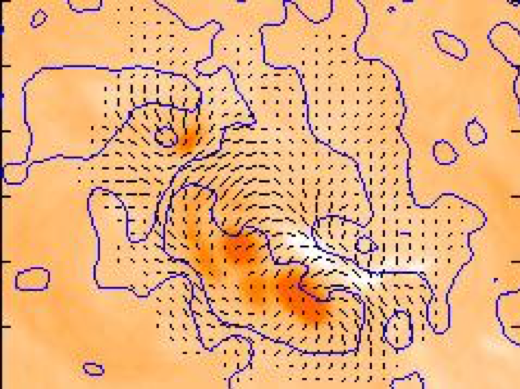
\includegraphics[width=3in]{osf2.png} 
	   \caption{Magnetic field structure around an active region of the sun}
	\end{figure}

In the image above, the solid blue lines account for the neutral lines in between areas of oppositely charged magnetic fields. Its direction and magnitude – the magnetic field vector components – are denoted by these many line segments. As is conventional understanding, the line segments loop directly across the blue neutral lines from an outward pointing i.e. positive magnetic region to an inward pointing i.e. negative magnetic region. And the length of an individual segment corresponds to the magnetic field strength of the given space. The solid blue neutral lines and the magnetic field line segments happens to fall on a sunspot cluster. And the most interesting find by the NASA-MSFC Vector Magnetograph is that the flares – the red regions – evidently falls on the areas where the magnetic field – the line segments orientation – is twisted in such a way that they point along the solid blue neutral lines. \\

\section{Why They Matter} 

Life on Earth has evolved to benefit from the sun as a primary source of energy. It thus cannot be absurd to avow that occurrences on our nearest star can impact Earth dwellers. This must certainly be the case with the most powerful of all solar phenomena, with solar flares. The intense X-ray emissions in a particularly large flare lasting for hours and recurring a number of times a day risks a communication blackout. This is because during such a flare, all high-frequency (HF) radio broadcasts such as shortwave Voice of America (VOA) and the British Broadcasting Corporation (BBC) traversing the ionosphere can be absorbed. This is especially so with radio wave frequencies ranging from 3 MHz (Mega-Hertz) to 30 MHz.\\

However, it is often not just the flares themselves, but also that they serve a visible harbinger producing highly energetic particles from the sun. \\

Astronauts beyond the protective magnetic field of the Earth would have to contend with the radiation hazards of chromosome damage and even cancer upon prolonged exposure. A significantly high doses could result in instant death. Similarly, satellites encircling the Earth in and above the low-Earth orbit could find their logic circuits for computer memory or control mechanisms upset. Solid state electronics high up could be severely impacted as energetic particles can also damage their space materials. Also, because these energetic particles cannot effectively be shielded off by the magnetic field of the Earth around its poles, they can reach the ionosphere in the regions causing positioning errors on transpolar pathways to the order of kilometers.  \\

As for the situation within the magnetic field of the Earth, there is the possibility of a geomagnetic storm occurring. Such storms are caused by inhomogeneities in the density, speed and magnetic field of the solar wind particles interacting with the magnetic field of the Earth. Some of these charged particles trapped above the atmosphere can flow around the Earth. This current would generate a magnetic field of its own that can be felt on the Earth. Terrestrial power grids have been disabled for extended periods of time by such storms. Should a satellite fall in their circuit, these could charge the satellite surface coating. The physical properties of the surface materials could be altered. Also, the energy of these particles deposited in the upper-atmosphere of the earth during a geomagnetic storm in turn can cause and ionospheric storm. This would again impact all radio communication, now in a larger frequency bracket, ranging from 3 KHz (Kilo-Hertz) to 30 GHz (Giga-Hertz). Many of our satellite communication systems operate in this range.    \\

These vulnerabilities in our global infrastructure upon which our reliance has steadily grown warrant predicting said flares to be one of the most important goals of solar physics. \\


\chapter{Applied Notions of Statistics}
		
\section{Probability}
The probability of obtaining a given outcome from a process can be interpreted to mean the relative frequency with which the said outcome would occur should the process be repeated under similar conditions and for a large number of times. But it is generally understood as a measure of the likelihood of an outcome being obtained when an experiment is performed. The probability measure of any event is generally assigned a value between 0 and 1 corresponding to the said event’s likelihood. The aforementioned process in which all the possible outcomes have already been identified is defined to be an experiment, and an event is the set for some of its possible outcomes. The experiment in our endeavor would thus be observing and measuring the radiation intensity from the sun thorough terrestrial observatories and artificial satellites. The event of interest then is the occurrence of solar flares.\\

Given S as our sample space i.e. the collection of all possible outcomes of an experiment, the probability of some event A, denoted Pr(A), must obey three specific axioms.

\begin{enumerate}
\item The probability of every event must be nonnegative, $Pr(A)\leq0$.
\item The probability of a certain event is $1$, $Pr(S)=1$. 
\item Events that cannot occur on the same time are defined to be disjoint or mutually exclusive events. For any sequence of such events $ \{A_1, A_2, A_3, \dots\}\subset S$, the probability of one or any other event in the sequence occurring is the sum of their individual probabilities, $ Pr(⁡\bigcup\limits_{i=1}^{\infty} A_{i})=\sum\limits_{i=1}^{\infty}Pr(A_i)$.
\end{enumerate}\\

It follows from the third axiom that the probability of an impossible event is 0, i.e. $Pr(\phi)=0$. And based on these axioms and their corollaries, we can have other general properties of probability.

\begin{enumerate}
\item For any event A, \textit{Pr(not event A)}$=Pr(A^c)=1–Pr(A)$.
\item If event A implies event B, i.e. $A\subseteq B$, then $Pr(A)\leq Pr(B)$. 
\item For every event A, $0\leq Pr(A)\leq 1$.
\item For any two events A and B, \\ \textit{Pr(A and not B) = Pr($A\cap B^c$) = Pr(A) – Pr($A\cap B$)}.
\item For any two events A and B, \\ \textit{Pr(A or B) = Pr($A\cup B$) =  Pr(A) + Pr(B) – Pr($A\cap B$)}.
\end{enumerate}\\

\section{Conditional Probability}

The probability of an event A after event B has occurred – denoted $Pr(A|B)$ – is defined to be the conditional probability of A given B. Provided $Pr(B) > 0$, it is determined as
\begin{center} 
\textit{Pr(A|B) = $\frac{Pr(A \cap  B)}{Pr(B)}$}. 
\end{center} \\

Conditional probabilities, just like probabilities, obey all of the above stated axioms. The conditional probability is not defined when $Pr(B) = 0$. \\

From this definition we derive the \textit{Multiplication Rule for Conditional Probabilities}. It states that if $Pr(B)> 0$, then 
\begin{center} 
\textit{Pr($A\cap B$) = Pr(B) Pr(A|B)},
\end{center} \\

and if $Pr(A)> 0$, then 
\begin{center} 
\textit{Pr($A\cap B$) = Pr(A) Pr(B|A)}.
\end{center}\\

Now suppose we consider k disjoint events $\{B_1, B_2, B_3, \dotsc, B_k\}$ such that they form a partition on of our sample space S i.e. $\bigcup\limits_{i=1}^k B_i  = S$, and $Pr(B_i) > 0$ for all $i = 1, 2, 3, \dotsc, k$. Then the \textit{Law of Total Probability} states that for every event A in S,
\begin{center} 
\textit{Pr(A) = $\sum\limits_{i=1}^k Pr(B_i) Pr(A|Bi)$}.
\end{center}\\

From this, we can also ascertain the \textit{Conditional Version of the Law of Total Probability} for another event C which states,
 \begin{center} 
\textit{Pr(A|C) = $\sum\limits_{i=1}^k Pr(B_{i}|C) Pr(A|B_i \cap C)$}.
 \end{center}\\

Sometimes, the occurrence of event B does not impact the probability of event A. This occurs when events A and B are independent and
\begin{enumerate}
\item \textit{Pr(A|B) = Pr(A)}.
\item \textit{Pr($A \cap  B$) = Pr(A) Pr(B)}.
\end{enmerate}\\

More generally, if we have a number of mutually independent events $B_1, B_2, B_3, \dotsc, B_k$, then for every corresponding subset of $j ( j = 2, 3, 4,\dotsc, k )$ of these events $B_{i,1}, B_{i,2}, \dotsc, B_{i,k}$,
\begin{center}
\textit{Pr($B_{i,1}\cap\dotsc\cap B_{i,j}$) = Pr($B_{i,1}) \dotsc Pr(B_{i,j}$)}.
\end{center}\\

For instance, for three independent events A, B and C, all of the following conditions are satisfied:
\begin{enumerate}
\item \textit{Pr($A\cap B$) = Pr(A) Pr(B)}.
\item \textit{Pr($A\cap C$) = Pr(A) Pr(C)}.
\item \textit{Pr($B\cap C$) = Pr(B) Pr(C)}.
\item \textit{Pr($A\cap B\cap C$) = Pr(A) Pr(B) Pr(C)}.
\end{enmerate}\\

Again, the conditional probability for such larger collections of independent events holds. For $B_1, B_2, B_3, \dotsc, B_k$ events such that $Pr(B_{i,1}\cap\dotsc\cap Bi,j) > 0$. Then $B_1, B_2, B_3,\dotsc, B_k$ are independent if and only if for every tow disjoint subsets ${i_1,\dotsc,1_m}$ and ${j_1,\dotsc,j_l}$ of ${1,\dotsc , k}$, then
\begin{center} 
$Pr(B_{i,1}\cap\dotsc\cap B_{i,m} | B_{j,1}\cap\dotsc\cap B_{j,l}) = Pr(B_{i,1} \cap\dotsc\cap B_{i,m})$.
\end{center} 

The said $k$ events are independent if and only if knowledge of some events occurring does not in any way impact the probability of any combination of the other events occurring.\\

To a lesser extent, the events $B_1, B_2, B_3, \dotsc, B_k$ are \textit{Conditionally Independent} given A if for its every subset $B_{i,1}, \dotsc , B_{i,j}$ where $j = 1, 2, \dotsc , k$ provided $Pr(A) > 0$ is 
\begin{center}
$Pr(B_{i,1} \cap \dotsc \cap B_{i,m} | A) = Pr(B_{i,1}|A) \dotsc Pr(B_{i,m}|A)$.
\end{center}\\

The definition also accordingly implies that events $B_1$ and $B_2$ are conditionally independent if and only if $Pr(B_2 | B_1 \cap A) = Pr(B_2 | A)$ given $Pr(B_1 | A) > 0$. \\

To determine the probability for some of these mutually independent events, say $B_1, B_2, B_3, \dotsc, B_k$, that partition the sample space S such that $Pr(B_j) > 0$ for $j = 1, \dotsc, k$, and A be an event such that $Pr(A) > 0$, then for $i = 1, 2, 3, \dotsc , k$,
\begin{center}
$Pr(B_i | A) =  \frac{Pr⁡(B_i )  Pr⁡(A | B_i)}{\sum\limits_{i=1}^k Pr(B_i)  Pr(A|B_i)}$.
\end{center}\\

This is according to \textit{Bayes’ Theorem} and can be derived from the very definition of conditional probability. \\

Now $Pr(B_i)$ is the Prior Probability because it is the probability of the event $B_i$ before the occurrence and impact of event A has been take into consideration. Correspondingly, the probability $Pr(B_i | A)$ would be the Posterior Probability of event $B_i$ since it is the probability of the event after the consequences of event A have also been taken into consideration. In our project, the phenomenological rules that govern solar flare occurrence. The posterior is then ascertained after taking all the additional data into consideration so as to obtain better flare predictability.  

\section{Random Variables & Distributions}

A random variable is a real-valued function defined on a sample space that assigns a numerical value to the outcome of a random experiment. For each random variable $X$ and each subset $R$ of real numbers, we can determine the probability that $X$ takes a value in $R$. The collection of all these probabilities is the distribution of $X$. The two categories of distributions and random variables we are interested in is either \textit{Discrete} or \textit{Continuous}.\\ 

A random variable $X$ has a $discrete distribution$ if it can only assume a finite or countably infinite positive values. $X$ is then referred to as a discrete random variable. The probability (mass) function or p.m.f. of $X$ is a real valued function $f$ for every real number $x$ where, 
\begin{center}
$f(x) = Pr(X = x)$.
\end{center}\\

The \textit{support of (distribution of) X} is the set of values in $X$ that have non-zero probability values. For any value that is not contained in $X$ i.e. $y \notin X$, $Pr(y) = 0$. Also, if $X = \{x_1, x_2, x_3, x_4, \dotsc \}$, 
\begin{center}
$\sum\limits_{i=1}^{\infty} f(x_i ) = 1$.
\end{center}\\

Similarly, a random variable $X$ is believed to have a \textit{continuous distribution} if there is a non-negative function $f$, defined on the real line, where for every bounded or non-bounded interval of real values, the probability that $X$ takes a value in the interval in the integral of $f$ over the interval. $X$ is then referred to as a $continuous random$ variable. Say there is a bounded and closed interval in $X$ i.e.$[a, b] \subseteq  X$, then 
\begin{center}
$Pr⁡(a≤ X ≤b) = \int\limits_{x=a}^{x=b} f(x)dx $.
\end{center}\\

Similarly, 

\begin{center}
$Pr⁡(x ≤ b)= \int\limits_{x = -\infty}^{x = b} f(x)dx$,\\ 
\end{center}\\

\begin{center}
and,
\end{center}

\begin{center}\\
$Pr⁡(x ≥ a)= \int\limits_{x = a}^{x = \infty} f(x) dx$.
\end{center}\\

The function $f$ from above is called the \textit{probability density function (p.d.f.) of X}. The \textit{support of (the distribution of) X} is the closure of the set $\{ x: f(x) > 0 $\}. One thing that sets a continuous distribution apart from a discrete distribution is that the former assigns probability 0 to any individual value.\\

In either case, we define the Cumulative Distribution Function (c.d.f.) F of a random variable X is the function,
\begin{center}
$F(x) = Pr(X ≤ x)$	for,	$-\infty < x < \infty$.
\end{center}\\

The distributions discussed so far have one random variable $X$. It is possible to generalize this concept to an arbitrary finite number n of random variables $X_1, X_2, X_3, \dotsc, X_n$. This joint distribution of more than two random variables is called \textit{multivariate distribution}, if $n = 2$ the it is referred to as \textit{bivariate distribution}. The \textit{joint distribution function (c.d.f.)} of $n$ random variables $X_1, X_2, X_3, \dotsc, X_n$ is the function $F$ whose value at every point $(x_1, x_2 \dotsc, x_n)$ in \textit{n-dimensional space $R^n$} specified as
\begin{center}
$F(x_1, \dotsc, x_n ) = Pr(X_1 \leq x_1, X_2 \leq x_2, \dotsc, X_n \leq x_n )$.
\end{center}\\

If the $n$ random variables $X_1, X_2, X_3, \dotsc, X_n$ have a \textit{discrete joint distribution}, the \textit{joint probability (mass) function} or \textit{p.m.f.} of $X_1, X_2, X_3, \dotsc , X_n$  is the function $f$ such that for every point $(x_1, x_2, … , x_n) \in R^n$ defined as,

\begin{center}
$f(x_1, …, x_n ) = Pr(X_1 = x_1, X_2 = x_2, \dotsc, X_n = x_n )$
\end{center}\\

\begin{center}
or,
\end{center}\\

\begin{center}
$f(x) = Pr(X = x)$
\end{center}\\

in vector notation where $X = (X_1, X_2, X_3, \dotsc, X_n )$, and $x = (x_1, x_2, x_3, \dotsc, x_n )$. Then for every subset $A \subset R^n$,
\begin{center}
$Pr(X \subset C) =\sum\limits_{\substack{x \in C}} f(x)$.
\end{center}\\

Similarly suppose the $n$ random variables $X_1, X_2, X_3, \dotsc, X_n$ have a \textit{continuous joint distribution}, then there exists a nonnegative function $f$ defined on $R^n$ such that for every subset $C \subset R^n$,
\begin{center}
$Pr[(X_1, \dotsc, X_n) \in C] = \idotsint f(x_1, \dotsc, x_n) dx_1 \dotsc. dx_n$,
\end{center}\\

provided the integral exists. The function $f$ serves as the \textit{joint probability density function (p.d.f.)} of $X_1, \dotsc, X_n$. And similarly as was the case with the vector notation for the joint discrete distribution, the continuous joint distribution in vector notation can be expressed as,

\begin{center}     
$Pr(X \in C) = \idotsint f(x)dx$.
\end{center}\\

And if the joint distribution of n random variables $X_1, \dotsc, X_n$ is known, then the \textit{Marginal  Distribution} – the probability distribution of each variable contained in the subset $(X_1, \dotsc, X_n)$ of $R^n$ – can be derived from the joint distribution above. For instance, the marginal p.d.f. $f_i$ of $X_i$ is specified at every value $x_i$ by the equation
\begin{center}
$f_i(x_i) = \int\limits_{-\infty}^{\infty} \dotsc	\int\limits_{-\infty}^{\infty} f(x_1, \dotsc, x_{i-1}, x_{i+1}, \dotsc, x_n) dx_1 … dx_{i-1} dx_{i+1} … dx_n$
\end{center}\\

integrated over n - 1 variables except $x_i$.\\ 

If the $n$ random variables $X_1, \dotsc, X_n$ are independent if, for every $n$ sets $C_1, C_2, \dotsc, C_n$ of real numbers, 
\begin{center} 
$Pr(X_1 \in C_1, X_1 \in C_1, …, X_n \in C_n) = Pr(X_1 \in C_1) Pr(X_2 \in C_2) \dots Pr(X_1 \in C_n)$.
\end{center}\\

And if $F_i$ were to denote the marginal c.d.f. of $X_i$  for $i = 1, 2, \dotsc, n$, then the variables $X_1, \dotsc, X_n$ are \textit{independent} if for any point $(x_1, \dotsc, x_n) \in R^n$, 
\begin{center}
$F(x_1, \dotsc, x_n) = F_1(x_1) F_2(x_2) \dots F_n(x_n)$. 
\end{center}\\

Similarlay, if the random variables $X_1, \dotsc, X_n$ have a continuous, discrete or a mixed joint distribution for which the joint p.d.f., joint p.m.f. or joint p.d.f. is $f$, and if $f_i$ is the marginal univariate p.d.f. or p.m.f. of $X_i$ $(i = 1, 2, …, n)$, then $X_1, \dotsc, X_n$ are independent if and only if their joint p.d.f./p.m.f. is the product of their $n$ individual p.d.f.’s or p.m.f.’s. So then for any point $(x_1, \dotsc, x_n) \in R^n$,
\begin{center}
$f(x_1, \dotsc, x_n) = f_1(x_1) f_2(x_2) f_3(x_3) \dots f_n(x_n)$. 
\end{center}\\

Suppose the random variables vector $X = (X_1, \dotsc, X_n)$ is divided into a $k$-dimensional random variable vector $Y$, and a $(n - k)$-dimensional variable random vector $Z$. Suppose also that the joint p.d.f. or p.m.f. of $(Y, Z)$ is $f_{y,z}$, and that the marginal distributions of $Y$ and $Z$ are $f_y$ and $f_z$ respectively, then their relationship with the conditional p.d.f. or p.m.f. $f_{y|z}$ of $Y$ given $Z = z$ is defined as:
\begin{center}
$f_{z|y} (z│y) = \frac{f_{(y|z)}(y|z) f_{z}(z)}{(f_{y}(y)}$.
\end{center}\\

The \textit{Multivariate Law of Total Probability}, \textit{Bayes’ Theorem} and the conditions given above provided $Z$ has a continuous joint distribution, then the marginal p.d.f. of $Y$ is
\begin{center}
$f_y(y) = \int\limits_{-\infty}^{\infty} \dotsc	\int\limits_{-\infty}^{\infty} f_{y|z}(y|z) f_z(z) dz$.
\end{center}\\

And suppose we have another random vector $W = w$ satisfying the prerequisite conditions, then 
\begin{center}
$f_y(y|w) = \int\limits_{-\infty}^{\infty} \dotsc \int\limits_{-\infty}^{\infty}  f_{y|z,w} (y|z, w) f_z(z|w) dz$,
\end{center}\\

where $f_{y|w}(y|w)$ is the conditional p.d.f. or p.m.f. of $Y$ given $W = w$, $f_{y|z,w}(y|z, w)$ is the conditional p.d.f. or p.m.f. of $Y$ given $(Z, W) = (z, w)$ and $f_z(z|w)$ is the conditional p.d.f. or p.m.f. of $Z$ given $W = w$. Then again we have the following result:
\begin{center}
$f_{(z|y,w)}(z|y, w) = \frac{f_{(y|z,w)}(y|z,w) f_z (z))}{f_{(y|w )}(y|w)}$.
\end{center}\\

And for the random variable vector $Z$ with joint p.d.f. or p.m.f. given by $f_z(z)$, suppose the random variables $X_1, \dotsc, X_n$ are all \textit{conditionally independent} given $Z$, then for all $z \in Z$ such that $f_z(z) > 0$, we have:
\begin{center} 
$f_{x,z}(x, z) = \prod\limits_{i=1}^n f_i (x_i|z)$,
\end{center}\\

where $f_{x,z}(x, z)$ is the conditional multivariate p.d.f. or p.m.f. of $X$ given $Z = z$ and $f_i(x_i|z)$ is the conditional univariate p.d.f. or p.m.f. of $X_i$ given $Z = z$. 

Now suppose $X$ has a discrete distribution with p.m.f. $f$, and let the other random variable be $Y = r(X)$, where $r$ is some function defined on the set of all permissible values for $X$. Then for any $y \in Y$, the p.m.f. of $Y$, $f_y(y)$ is defined as:
\begin{center}
$f_y(y) = Pr(Y = y) = Pr[r(X) = y] = \sum\limits_{\substack{x:r(x)  = y}} f(x)$.
\end{center}\\

The result can be generalized to m functions $Y_1, Y_2, … , Y_m$ where $Y_i = r_i(X)$ for $i = {1, 2, \dotsc, m}$. Then the joint p.d.f. of $Y_1, Y_2, \dotsc , Y_m$ for any specified point $y = (y_1, y_2, … , y_m)$ is determined by,
\begin{center}
$f_y(y) = \sum\limits_{\substack{x \in A}} f(x_1, x_2, \dotsc ,x_n)$,
\end{center}\\

where $A$ is the set of all possible points $x = (x_1, x_2, \dotsc , x_n)$ satisfying the $m$ functions.\\
  
Now suppose $X$ has a continuous distribution with p.d.f. $f$ and let $Y = r(X)$. Then for each real value $y$, the c.d.f. $G(y)$ of $Y$ is determined via. 
\begin{center}
$G(y) = Pr(Y \leq y) = Pr[r(X) \leq y] =  \int\limits_{\substack{x:r(x)  ≤ y}} f(x) dx$.
\end{center}
And should the random variable $Y$ itself also have a continuous distribution, then its p.d.f. at every point $y \in Y$ where $G$ is differentiable can be obtained by from the expression: 
\begin{center}
$g(y) = G'(y) = \frac{d}{dy} G(y)$.
\end{center}






\subsection{References and Labels}
Sometimes you'd like to refer to a table or figure, e.g. you can see in Figure \ref{subd2} that you can rotate figures . Start by labeling your figure or table with the label command (\verb=\label{labelvariable}=) below the caption (see the chapter on graphics and tables for examples). Then when you would like to refer to the table or figure, use the ref command (\verb=\ref{labelvariable}=). Make sure your label variables are unique; you can't have two elements named ``default." Also, since the reference command only puts the figure or table number, you will have to put  ``Table" or ``Figure" as appropriate, as seen in the following examples:


\chapter{Wheatland's Bayesian Approach}

\section{The Priors}

\subsection{The Phenomenological Rules}

By phenomenological rules we are referring specifically to the laws governing the various aspects of solar flare occurrence based on observations from solar telescopes. The first rule proposed by James F. Drake in 1971 suggests that flare events follow a power-law size distribution where by ‘size’ refers to the peak flux in soft X-ray or extreme ultraviolet in terms of estimated energy. Drake’s flare \textit{'Frequency-Size Distribution'} would translate as:
\begin{center}
\begin{equation} \label{FreqSize}
$ N(S) = AS^{-\gamma}\qquad$
\end{equation}
\end{center}\\

where ‘N(S)’ is the distribution for the number of flare events per unit size ‘S’ and per unit time, with constants ‘$A$’ and ‘$\gamma$’. The constant ‘$A$’ is the overall flaring rate, and the exact power-law index ‘$\gamma$’ is a constant estimated by Aschwanden et al. in 2000 to be $1.8$ and certainly less than $2$. But it was already understood to have a constant value lying somewhere in between $1.5$ and $2$ according to Crosby et al. in 1993. This was so that the mean flare size is finite. Bai in 1993 uncovered some indication that the power-law index varies with the solar cycle. But Wheatland in 2000 revealed its value to be mostly constant irrespective of the active region under consideration.\\

There are however numerable inconsistencies in the model proposed above.\\

As noted above, Bai in 1993 showed that the occurrence frequency of flares as a function of hard X-ray peak count rate varies. The power-law index of size distribution was found to change with time and with the phase of a 154-day periodicity. Kucera et al. in 1997 found fewer high count rate flares (i.e. $\leq$ 104 counts per second and size above 60 keV) from regions with small sunspot areas (ranging from 0 to 500 microhemispheres) than the power-law extrapolation from the frequency distribution of flares with peak rates higher than 50 counts per second above 60 keV. A lower proportion low-energy events was seen in large complex regions than in smaller, simpler regions. Furthermore, Ian Sammis in 1999 discovered that all active regions do not share a common power-law distribution i.e. local distribution was not consistent with the global distribution. Finally, Wheatland in 2000 studied the small and highly active region 11029 and noted its departure from the power-law behavior above 10$Wm^{-2}$ to 6$Wm^{-2}$. Wheatland attributed this to the small active region having a finite amount energy. \\

Another candidate governs the \textit{‘Waiting-Time Distribution’} i.e. the way flares occur in time. It was first modeled as a Poisson process in time by Rosner and Vaiana in 1978. The model assumes individual flares to be independent of each other, and the distribution for events occurring between times $\tau$ and $\tau$ + d$\tau$  i.e. $P(\tau$ )d\tau$, where

\begin{center}
\begin{equation} \label{WaitTime}
$ P(\tau) = \lambda e^{-\lambda\tau}\qquad$
\end{equation}
\end{center}\\ 
  
where $'\lambda'$ is the constant mean rate of occurrence or frequency. We note here that the waiting-times of the Poisson process follows an exponential distribution.\\

But several observations were shown to conflict with the given poisson model. Biesecker in 1994 found the waiting-time distribution for hard X-rays to be consistent with a time-dependent Poisson process. Whereas the waiting-time distribution was shown to obey follow the power law via. statistical analysis of observational data by Dennis in 1985, and by Crosby et al. and Pearce et al. independently 1993. Furthermore, using data observed by GOES sensors between 1976 and 1996, Boffetta et al. in 1999 revealed that for waiting times longer than 10 hours, it follows a power-law. But then Wheatland in 2000 showed that the distribution of GOES flares is consistent with a time-dependent Poisson process. A new phenomenological rule for solar flares, that the time distribution of rates of the flares averaged over several solar cycles is approximately exponential, was also presented.\\

The Poisson model was then restructured into a time-dependent Poisson process by Wheatland and Litvinenko in 2002. Independent events with time varying mean rate $'\lambda(\tau)’$ was accounted for. And for a varying mean rate given by some distribution, say $‘f(\tau)’$, the corresponding waiting-time distribution between times $\tau$ and $\tau$+$d\tau$ i.e. P($\tau)d\tau$, where 

\begin{center}
\begin{equation} \label{NewWaitTime}
$ P(\tau) = \frac{1}{\lambda} \int\limits_{0}^{\infty} f(\lambda) \lambda^{2} e^{-\lambda\tau} d\lambda \qquad$
\end{equation}
\end{center}\\ 

The GOES data found the distribution for the slowly varying $‘f(\lambda)’$ approximation to be valid. But then again, they also noted the deviation in the power-law index with the solar cycle variation. That very year, Moon et al. studied sympathetic Coronal Mass Ejections. Sympathetic events are solar eruptions and flares that occur almost simultaneously in one complex region or in different active regions with a physical link. Although the results indicated that sympathetic events are rarer than their anti-sympathetic counterparts, they did find a candidate sympathetic event pair where the first event may trigger the second flare occurrence. This starkly contradicts the central tenet of a Poisson process where events are assumed to be independent of each other. \\




\chapter{Neural Networks}
	
\section{The Elements}
It is easy to refer to anything within your document using the \texttt{label} and \texttt{ref} tags.  Labels must be unique and shouldn't use any odd characters; generally sticking to letters and numbers (no spaces) should be fine. Put the label on whatever you want to refer to, and put the reference where you want the reference. \LaTeX\ will keep track of the chapter, section, and figure or table numbers for you. 
	
\section{In Solar Forecasting}
	Of course you will need to cite things, and you will probably accumulate an armful of sources. This is why BibTeX was created. For more information about BibTeX and bibliographies, see our CUS site (\url{web.reed.edu/cis/help/latex/index.html})\footnote{\cite{reedweb:2007}}. There are three pages on this topic: {\it bibtex} (which talks about using BibTeX, at \url{/latex/bibtex.html}), {\it bibtexstyles} (about how to find and use the bibliography style that best suits your needs, at \url{/latex/bibtexstyles.html}) and {\it bibman} (which covers how to make and maintain a bibliography by hand, without BibTeX, at at \url{/latex/bibman.html}). The last page will not be useful unless you have only a few sources. There used to be APA stuff here, but we don't need it since I've fixed this with my apa-good natbib style file.
	

\chapter{Sunspots: Possible Precursors?}	
	
\section{Understanding Sunspots}
It is easy to refer to anything within your document using the \texttt{label} and \texttt{ref} tags.  Labels must be unique and shouldn't use any odd characters; generally sticking to letters and numbers (no spaces) should be fine. Put the label on whatever you want to refer to, and put the reference where you want the reference. \LaTeX\ will keep track of the chapter, section, and figure or table numbers for you. 
	
\section{Predicting Sunspots}
	Of course you will need to cite things, and you will probably accumulate an armful of sources. This is why BibTeX was created. For more information about BibTeX and bibliographies, see our CUS site (\url{web.reed.edu/cis/help/latex/index.html})\footnote{\cite{reedweb:2007}}. There are three pages on this topic: {\it bibtex} (which talks about using BibTeX, at \url{/latex/bibtex.html}), {\it bibtexstyles} (about how to find and use the bibliography style that best suits your needs, at \url{/latex/bibtexstyles.html}) and {\it bibman} (which covers how to make and maintain a bibliography by hand, without BibTeX, at at \url{/latex/bibman.html}). The last page will not be useful unless you have only a few sources. There used to be APA stuff here, but we don't need it since I've fixed this with my apa-good natbib style file.

\section{Sunspots & Solar Flares}
	Of course you will need to cite things, and you will probably accumulate an armful of sources. This is why BibTeX was created. For more information about BibTeX and bibliographies, see our CUS site (\url{web.reed.edu/cis/help/latex/index.html})\footnote{\cite{reedweb:2007}}. There are three pages on this topic: {\it bibtex} (which talks about using BibTeX, at \url{/latex/bibtex.html}), {\it bibtexstyles} (about how to find and use the bibliography style that best suits your needs, at \url{/latex/bibtexstyles.html}) and {\it bibman} (which covers how to make and maintain a bibliography by hand, without BibTeX, at at \url{/latex/bibman.html}). The last page will not be useful unless you have only a few sources. There used to be APA stuff here, but we don't need it since I've fixed this with my apa-good natbib style file.






\chapter{Useful Codes:}
	
	
\section{References, Labels, Custom Commands and Footnotes}
It is easy to refer to anything within your document using the \texttt{label} and \texttt{ref} tags.  Labels must be unique and shouldn't use any odd characters; generally sticking to letters and numbers (no spaces) should be fine. Put the label on whatever you want to refer to, and put the reference where you want the reference. \LaTeX\ will keep track of the chapter, section, and figure or table numbers for you. 

\subsection{References and Labels}
Sometimes you'd like to refer to a table or figure, e.g. you can see in Figure \ref{subd2} that you can rotate figures . Start by labeling your figure or table with the label command (\verb=\label{labelvariable}=) below the caption (see the chapter on graphics and tables for examples). Then when you would like to refer to the table or figure, use the ref command (\verb=\ref{labelvariable}=). Make sure your label variables are unique; you can't have two elements named ``default." Also, since the reference command only puts the figure or table number, you will have to put  ``Table" or ``Figure" as appropriate, as seen in the following examples:

 As I showed in Table \ref{inheritance} many factors can be assumed to follow from inheritance. Also see the Figure \ref{subd} for an illustration.
 
\subsection{Custom Commands}\label{commands}
Are you sick of writing the same complex equation or phrase over and over? 

The custom commands should be placed in the preamble, or at least prior to the first usage of the command. The structure of the \verb=\newcommand= consists of the name of the new command in curly braces, the number of arguments to be made in square brackets and then, inside a new set of curly braces, the command(s) that make up the new command. The whole thing is sandwiched inside a larger set of curly braces. 

% Note: you cannot use numbers in your commands!
\newcommand{\hydro}{H$_2$SO$_4$}

In other words, if you want to make a shorthand for H$_2$SO$_4$, which doesn't include an argument, you would write: \verb=\newcommand{\hydro}{H$_2$SO$_4$}= and then when you needed  to use the command you would type \verb=\hydro=. (sans verb and the equals sign brackets, if you're looking at the .tex version). For example: \hydro

\subsection{Footnotes and Endnotes}
	You might want to footnote something.\footnote{footnote text} Be sure to leave no spaces between the word immediately preceding the footnote command and the command itself. The footnote will be in a smaller font and placed appropriately. Endnotes work in much the same way. More information can be found about both on the CUS site.
	
\section{Bibliographies}
	Of course you will need to cite things, and you will probably accumulate an armful of sources. This is why BibTeX was created. For more information about BibTeX and bibliographies, see our CUS site (\url{web.reed.edu/cis/help/latex/index.html})\footnote{\cite{reedweb:2007}}. There are three pages on this topic: {\it bibtex} (which talks about using BibTeX, at \url{/latex/bibtex.html}), {\it bibtexstyles} (about how to find and use the bibliography style that best suits your needs, at \url{/latex/bibtexstyles.html}) and {\it bibman} (which covers how to make and maintain a bibliography by hand, without BibTeX, at at \url{/latex/bibman.html}). The last page will not be useful unless you have only a few sources. There used to be APA stuff here, but we don't need it since I've fixed this with my apa-good natbib style file.
	
\subsection{Tips for Bibliographies}
\begin{enumerate}
\item Like with thesis formatting, the sooner you start compiling your bibliography for something as large as thesis, the better. Typing in source after source is mind-numbing enough; do you really want to do it for hours on end in late April? Think of it as procrastination.
\item The cite key (a citation's label) needs to be unique from the other entries.
\item When you have more than one author or editor, you need to separate each author's name by the word ``and'' e.g.\\ \verb+Author = {Noble, Sam and Youngberg, Jessica},+.
\item Bibliographies made using BibTeX (whether manually or using a manager) accept LaTeX markup, so you can italicize and add symbols as necessary.
\item To force capitalization in an article title or where all lowercase is generally used, bracket the capital letter in curly braces.
\item You can add a Reed Thesis citation\footnote{\cite{noble:2002}} option. The best way to do this is to use the phdthesis type of citation, and use the optional ``type'' field to enter ``Reed thesis'' or ``Undergraduate thesis''. Here's a test of Chicago, showing the second cite in a row\footnote{\cite{noble:2002}} being different. Also the second time not in a row\footnote{\cite{reedweb:2007}} should be different. Of course in other styles they'll all look the same.
\end{enumerate}
\section{Anything else?}
If you'd like to see examples of other things in this template, please contact CUS (email cus@reed.edu) with your suggestions. We love to see people using \LaTeX\ for their theses, and are happy to help.


\chapter{Mathematics and Science}	
\section{Math}
	\TeX\ is the best way to typeset mathematics. Donald Knuth designed \TeX\ when he got frustrated at how long it was taking the typesetters to finish his book, which contained a lot of mathematics. 
	
	If you are doing a thesis that will involve lots of math, you will want to read the following section which has been commented out. If you're not going to use math, skip over this next big red section. (It's red in the .tex file but does not show up in the .pdf.)
%	
%% MATH and PHYSICS majors: Uncomment the following section	
%	$$\sum_{j=1}^n (\delta\theta_j)^2 \leq {{\beta_i^2}\over{\delta_i^2 + \rho_i^2}}
%\left[ 2\rho_i^2 + {\delta_i^2\beta_i^2\over{\delta_i^2 + \rho_i^2}} \right] \equiv \omega_i^2
%$$

%From Informational Dynamics, we have the following (Dave Braden):

%After {\it n} such encounters the posterior density for $\theta$ is

%$$
%\pi(\theta|X_1< y_1,\dots,X_n<y_n) \varpropto \pi(\theta) \prod_{i=1}^n\int_{-\infty}^{y_i}
%   \exp\left(-{(x-\theta)^2\over{2\sigma^2}}\right)\ dx
%$$

%

%Another equation:

%$$\det\left|\,\begin{matrix}%
%c_0&c_1\hfill&c_2\hfill&\ldots&c_n\hfill\cr
%c_1&c_2\hfill&c_3\hfill&\ldots&c_{n+1}\hfill\cr
%c_2&c_3\hfill&c_4\hfill&\ldots&c_{n+2}\hfill\cr
%\,\vdots\hfill&\,\vdots\hfill&
%  \,\vdots\hfill&&\,\vdots\hfill\cr
%c_n&c_{n+1}\hfill&c_{n+2}\hfill&\ldots&c_{2n}\hfill\cr
%\end{matrix}\right|>0$$

%
%Lapidus and Pindar, Numerical Solution of Partial Differential Equations in Science and
%Engineering.  Page 54

%$$
%\int_t\left\{\sum_{j=1}^3 T_j \left({d\phi_j\over dt}+k\phi_j\right)-kT_e\right\}w_i(t)\ dt=0,
%   \qquad\quad i=1,2,3. 
%$$

%L\&P  Galerkin method weighting functions.  Page 55

%$$
%\sum_{j=1}^3 T_j\int_0^1\left\{{d\phi_j\over dt} + k\phi_j\right\} \phi_i\ dt 
%   = \int_{0}^1k\,T_e\phi_idt, \qquad i=1,2,3 $$
%   
%Another L\&P (p145)

%$$
%\int_{-1}^1\!\int_{-1}^1\!\int_{-1}^1 f\big(\xi,\eta,\zeta\big) 
%   = \sum_{k=1}^n\sum_{j=1}^n\sum_{i=1}^n w_i w_j w_k f\big( \xi,\eta,\zeta\big).
%$$

%Another L\&P (p126)

%$$
%\int_{A_e} (\,\cdot\,) dx dy = \int_{-1}^1\!\int_{-1}^1 (\,\cdot\,) \det[J] d\xi d\eta.
%$$

\section{Chemistry 101: Symbols}
Chemical formulas will look best if they are not italicized. Get around math mode's automatic italicizing by using the argument \verb=$\mathrm{formula here}$=, with your formula inside the curly brackets.

So, $\mathrm{Fe_2^{2+}Cr_2O_4}$ is written \verb=$\mathrm{Fe_2^{2+}Cr_2O_4}$=\\
Exponent or Superscript: O$^{-}$\\
Subscript: CH$_{4}$\\

To stack numbers or letters as in $\mathrm{Fe_2^{2+}}$, the subscript is defined first, and then the superscript is defined.\\
Angstrom: {\AA}\\
Bullet: CuCl $\bullet$ 7H${_2}$O\\
Double Dagger: \ddag \/\\
Delta: $\Delta$\\
Reaction Arrows: $\longrightarrow$ or  $\xrightarrow{solution}$\\
Resonance Arrows: $\leftrightarrow$\\
Reversible Reaction Arrows: $\rightleftharpoons$ or $\xrightleftharpoons[ ]{solution}$ (the latter requires the chemarr package)\\


\subsection{Typesetting reactions}
You may wish to put your reaction in a figure environment, which means that LaTeX will place the reaction where it fits and you can have a figure legend if desired:
\begin{figure}[htbp]
\begin{center}
$\mathrm{C_6H_{12}O_6  + 6O_2} \longrightarrow \mathrm{6CO_2 + 6H_2O}$
\caption{Combustion of glucose}
\label{combustion of glucose}
\end{center}
\end{figure}

\subsection{Other examples of reactions}
$\mathrm{NH_4Cl_{(s)}} \rightleftharpoons \mathrm{NH_{3(g)}+HCl_{(g)}}$\\
$\mathrm{MeCH_2Br + Mg} \xrightarrow[below]{above} \mathrm{MeCH_2\bullet Mg \bullet Br}$

\section{Physics}

Many of the symbols you will need can be found on the math page (\url{http://web.reed.edu/cis/help/latex/math.html}) and the Comprehensive \LaTeX\ Symbol Guide (enclosed in this template download).  You may wish to create custom commands for commonly used symbols, phrases or equations, as described in Chapter \ref{commands}.

\section{Biology}
You will probably find the resources at \url{http://www.lecb.ncifcrf.gov/~toms/latex.html} helpful, particularly the links to bsts for various journals. You may also be interested in TeXShade for nucleotide typesetting (\url{http://homepages.uni-tuebingen.de/beitz/txe.html}).  Be sure to read the proceeding chapter on graphics and tables, and remember that the thesis template has versions of Ecology and Science bsts which support webpage citation formats. 

\chapter{Tables and Graphics}

\section{Tables}
	The following section contains examples of tables, most of which have been commented out for brevity. (They will show up in the .tex document in red, but not at all in the .pdf). For more help in constructing a table (or anything else in this document), please see the LaTeX pages on the CUS site. 

\begin{table}[htbp] % begins the table floating environment. This enables LaTeX to fit the table where it works best and lets you add a caption.
\caption[Correlation of Inheritance Factors between Parents and Child]{Correlation of Inheritance Factors between Parents and Child} 
% The words in square brackets of the caption command end up in the Table of Tables. The words in curly braces are the caption directly over the table.
\begin{center} 
% makes the table centered
\begin{tabular}{c c c c} 
% the tabular environment is used to make the table itself. The {c c c c} specify that the table will have four columns and they will all be center-aligned. You can make the cell contents left aligned by replacing the Cs with Ls or right aligned by using Rs instead. Add more letters for more columns, and pipes (the vertical line above the backslash) for vertical lines. Another useful type of column is the p{width} column, which forces text to wrap within whatever width you specify e.g. p{1in}. Text will wrap badly in narrow columns though, so beware.
\toprule % a horizontal line, slightly thicker than \hline, depends on the booktabs package
  Factors &  Correlation between Parents \& Child & Inherited \\ % the first row of the table. Separate columns with ampersands and end the line with two backslashes. An environment begun in one cell will not carry over to adjacent rows.
  \midrule % another horizontal line
	Education 				& -0.49 & Yes 	 \\ % another row
	Socio-Economic Status 	& 0.28 	& Slight \\
	Income 					& 0.08 	& No	 \\
	Family Size 			& 0.19 	& Slight \\
	Occupational Prestige 	& 0.21 	& Slight \\
\bottomrule % yet another horizontal line
\end{tabular}
\end{center}
\label{inheritance} % labels are useful when you have more than one table or figure in your document. See our online documentation for more on this.
\end{table}

	\clearpage 
%% \clearpage ends the page, and also dumps out all floats. 
%% Floats are things like tables and figures.

If you want to make a table that is longer than a page, you will want to use the longtable environment. Uncomment the table below to see an example, or see our online documentation.

%% An example of a long table, with headers that repeat on each subsequent page: Results from the summers of 1998 and 1999 work at Reed College done by Grace Brannigan, Robert Holiday and Lien Ngo in 1998 and Kate Brown and Christina Inman in 1999.

	\begin{longtable}{||c|c|c|c||}
	 	\caption[Chromium Hexacarbonyl Data Collected in 1998--1999]{Chromium Hexacarbonyl Data Collected in 1998--1999}\\ \hline
	    	  \multicolumn{4}{||c||}{Chromium Hexacarbonyl} \\\hline
		   State & Laser wavelength & Buffer gas & Ratio of $\frac{\textrm{Intensity
at vapor pressure}}{\textrm{Intensity at 240 Torr}}$ \\ \hline
		  \endfirsthead
		\hline     State & Laser wavelength & Buffer gas & Ratio of
$\frac{\textrm{Intensity at vapor pressure}}{\textrm{Intensity at 240 Torr}}$\\
\hline
		    \endhead

	    $z^{7}P^{\circ}_{4}$ & 266 nm & Argon & 1.5 \\\hline
	    $z^{7}P^{\circ}_{2}$ & 355 nm & Argon & 0.57 \\\hline
	    $y^{7}P^{\circ}_{3}$ & 266 nm & Argon & 1 \\\hline
	    $y^{7}P^{\circ}_{3}$ & 355 nm & Argon & 0.14 \\\hline
	    $y^{7}P^{\circ}_{2}$ & 355 nm & Argon & 0.14 \\\hline
	    $z^{5}P^{\circ}_{3}$ & 266 nm & Argon & 1.2 \\\hline
	    $z^{5}P^{\circ}_{3}$ & 355 nm & Argon & 0.04 \\\hline
	    $z^{5}P^{\circ}_{3}$ & 355 nm & Helium & 0.02 \\\hline
	    $z^{5}P^{\circ}_{2}$ & 355 nm & Argon & 0.07 \\\hline
	    $z^{5}P^{\circ}_{1}$ & 355 nm & Argon & 0.05 \\\hline
	    $y^{5}P^{\circ}_{3}$ & 355 nm & Argon & 0.05, 0.4 \\\hline
	    $y^{5}P^{\circ}_{3}$ & 355 nm & Helium & 0.25 \\\hline
	    $z^{5}F^{\circ}_{4}$ & 266 nm & Argon & 1.4 \\\hline
	    $z^{5}F^{\circ}_{4}$ & 355 nm & Argon & 0.29 \\\hline
	    $z^{5}F^{\circ}_{4}$ & 355 nm & Helium & 1.02 \\\hline
	    $z^{5}D^{\circ}_{4}$ & 355 nm & Argon & 0.3 \\\hline
	    $z^{5}D^{\circ}_{4}$ & 355 nm & Helium & 0.65 \\\hline
	    $y^{5}H^{\circ}_{7}$ & 266 nm & Argon & 0.17 \\\hline
	    $y^{5}H^{\circ}_{7}$ & 355 nm & Argon & 0.13 \\\hline
	    $y^{5}H^{\circ}_{7}$ & 355 nm & Helium & 0.11 \\\hline
	    $a^{5}D_{3}$ & 266 nm & Argon & 0.71 \\\hline
	    $a^{5}D_{2}$ & 266 nm & Argon & 0.77 \\\hline
	    $a^{5}D_{2}$ & 355 nm & Argon & 0.63 \\\hline
	    $a^{3}D_{3}$ & 355 nm & Argon & 0.05 \\\hline
	    $a^{5}S_{2}$ & 266 nm & Argon & 2 \\\hline
	    $a^{5}S_{2}$ & 355 nm & Argon & 1.5 \\\hline
	    $a^{5}G_{6}$ & 355 nm & Argon & 0.91 \\\hline
	    $a^{3}G_{4}$ & 355 nm & Argon & 0.08 \\\hline
	    $e^{7}D_{5}$ & 355 nm & Helium & 3.5 \\\hline
	    $e^{7}D_{3}$ & 355 nm & Helium & 3 \\\hline
	    $f^{7}D_{5}$ & 355 nm & Helium & 0.25 \\\hline
	    $f^{7}D_{5}$ & 355 nm & Argon & 0.25 \\\hline
	    $f^{7}D_{4}$ & 355 nm & Argon & 0.2 \\\hline
	    $f^{7}D_{4}$ & 355 nm & Helium & 0.3 \\\hline
	    \multicolumn{4}{||c||}{Propyl-ACT} \\\hline
%	    State & Laser wavelength & Buffer gas & Ratio of $\frac{\textrm{Intensity
%at vapor pressure}}{\textrm{Intensity at 240 Torr}}$\\ \hline
	    $z^{7}P^{\circ}_{4}$ & 355 nm & Argon & 1.5 \\\hline
	    $z^{7}P^{\circ}_{3}$ & 355 nm & Argon & 1.5 \\\hline
	    $z^{7}P^{\circ}_{2}$ & 355 nm & Argon & 1.25 \\\hline
	    $z^{7}F^{\circ}_{5}$ & 355 nm & Argon & 2.85 \\\hline
	    $y^{7}P^{\circ}_{4}$ & 355 nm & Argon & 0.07 \\\hline
	    $y^{7}P^{\circ}_{3}$ & 355 nm & Argon & 0.06 \\\hline
	    $z^{5}P^{\circ}_{3}$ & 355 nm & Argon & 0.12 \\\hline
	    $z^{5}P^{\circ}_{2}$ & 355 nm & Argon & 0.13 \\\hline
	    $z^{5}P^{\circ}_{1}$ & 355 nm & Argon & 0.14 \\\hline
	    \multicolumn{4}{||c||}{Methyl-ACT} \\\hline
%	    State & Laser wavelength & Buffer gas & Ratio of $\frac{\textrm{Intensity
% at vapor pressure}}{\textrm{Intensity at 240 Torr}}$\\ \hline
	    $z^{7}P^{\circ}_{4}$ & 355 nm & Argon & 1.6, 2.5 \\\hline
	    $z^{7}P^{\circ}_{4}$ & 355 nm & Helium & 3 \\\hline
	    $z^{7}P^{\circ}_{4}$ & 266 nm & Argon & 1.33 \\\hline
	    $z^{7}P^{\circ}_{3}$ & 355 nm & Argon & 1.5 \\\hline
	    $z^{7}P^{\circ}_{2}$ & 355 nm & Argon & 1.25, 1.3 \\\hline
	    $z^{7}F^{\circ}_{5}$ & 355 nm & Argon & 3 \\\hline
	    $y^{7}P^{\circ}_{4}$ & 355 nm & Argon & 0.07, 0.08 \\\hline
	    $y^{7}P^{\circ}_{4}$ & 355 nm & Helium & 0.2 \\\hline
	    $y^{7}P^{\circ}_{3}$ & 266 nm & Argon & 1.22 \\\hline
	    $y^{7}P^{\circ}_{3}$ & 355 nm & Argon & 0.08 \\\hline
	    $y^{7}P^{\circ}_{2}$ & 355 nm & Argon & 0.1 \\\hline
	    $z^{5}P^{\circ}_{3}$ & 266 nm & Argon & 0.67 \\\hline
	    $z^{5}P^{\circ}_{3}$ & 355 nm & Argon & 0.08, 0.17 \\\hline
	    $z^{5}P^{\circ}_{3}$ & 355 nm & Helium & 0.12 \\\hline
	    $z^{5}P^{\circ}_{2}$ & 355 nm & Argon & 0.13 \\\hline
	    $z^{5}P^{\circ}_{1}$ & 355 nm & Argon & 0.09 \\\hline
	    $y^{5}H^{\circ}_{7}$ & 355 nm & Argon & 0.06, 0.05 \\\hline
	    $a^{5}D_{3}$ & 266 nm & Argon & 2.5 \\\hline
	    $a^{5}D_{2}$ & 266 nm & Argon & 1.9 \\\hline
	    $a^{5}D_{2}$ & 355 nm & Argon & 1.17 \\\hline
	    $a^{5}S_{2}$ & 266 nm & Argon & 2.3 \\\hline
	    $a^{5}S_{2}$ & 355 nm & Argon & 1.11 \\\hline
	    $a^{5}G_{6}$ & 355 nm & Argon & 1.6 \\\hline
	    $e^{7}D_{5}$ & 355 nm & Argon & 1 \\\hline

		\end{longtable}

   
   \section{Figures}
   
	If your thesis has a lot of figures, \LaTeX\ might behave better for you than that other word processor.  One thing that may be annoying is the way it handles ``floats'' like tables and figures. \LaTeX\ will try to find the best place to put your object based on the text around it and until you're really, truly done writing you should just leave it where it lies.   There are some optional arguments to the figure and table environments to specify where you want it to appear; see the comments in the first figure.

	If you need a graphic or tabular material to be part of the text, you can just put it inline. If you need it to appear in the list of figures or tables, it should be placed in the floating environment. 
	
	To get a figure from StatView, JMP, SPSS or other statistics program into a figure, you can print to pdf or save the image as a jpg or png. Precisely how you will do this depends on the program: you may need to copy-paste figures into Photoshop or other graphic program, then save in the appropriate format.
	
	Below we have put a few examples of figures. For more help using graphics and the float environment, see our online documentation.
	
	And this is how you add a figure with a graphic:
	\begin{figure}[h]
	% the options are h = here, t = top, b = bottom, p = page of figures.
	% you can add an exclamation mark to make it try harder, and multiple
	% options if you have an order of preference, e.g.
	% \begin{figure}[h!tbp]
	   
	       \centering
	    % DO NOT ADD A FILENAME EXTENSION TO THE GRAPHIC FILE
	    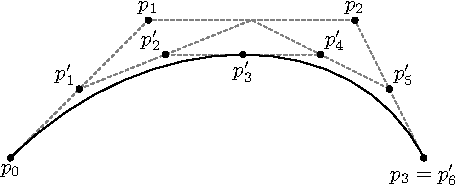
\includegraphics{subdivision}
	     \caption{A Figure}
	 \label{subd}
	\end{figure}

\clearpage %% starts a new page and stops trying to place floats such as tables and figures

\section{More Figure Stuff}
You can also scale and rotate figures.
 	\begin{figure}[h!]
	   
	       \centering
	    % DO NOT ADD A FILENAME EXTENSION TO THE GRAPHIC FILE
	    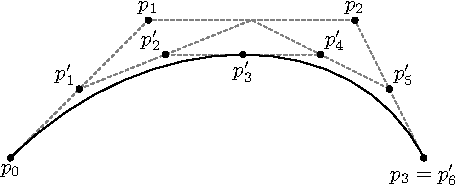
\includegraphics[scale=0.5,angle=180]{subdivision}
	    % if your figure shows up not where you want it, it may just be too big to fit. You can use the scale argument to shrink it, e.g. scale=0.85 is 85 percent of the original size. 
	     \caption{A Smaller Figure, Flipped Upside Down}
	 \label{subd2}
	\end{figure}

\section{Even More Figure Stuff}
With some clever work you can crop a figure, which is handy if (for instance) your EPS or PDF is a little graphic on a whole sheet of paper. The viewport arguments are the lower-left and upper-right coordinates for the area you want to crop.

 	\begin{figure}[h!]
	    	       \centering
	    % DO NOT ADD A FILENAME EXTENSION TO THE GRAPHIC FILE
	   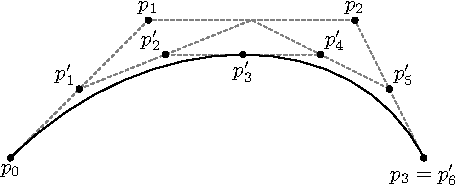
\includegraphics[clip=true, viewport=.0in .0in 1in 1in]{subdivision}
	    \caption{A Cropped Figure}
	 \label{subd3}
	\end{figure}
	
      \subsection{Common Modifications}
      The following figure features the more popular changes thesis students want to their figures. This information is also on the web at \url{web.reed.edu/cis/help/latex/graphics.html}.
    %\renewcommand{\thefigure}{0.\arabic{figure}} 	% Renumbers the figure to the type 0.x
    %\addtocounter{figure}{4} 						% starts the figure numbering at 4
    \begin{figure}[htbp]
    \begin{center}
   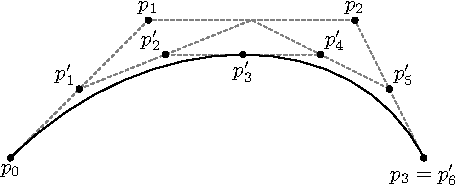
\includegraphics[scale=0.5]{subdivision}
    \caption[Subdivision of arc segments]{\footnotesize{Subdivision of arc segments. You can see that $ p_3 = p_6^\prime$.}} %the special ToC caption is in square brackets. The \footnotesize makes the figure caption smaller
    \label{barplot}
    \end{center}
    \end{figure} 

\chapter*{Conclusion}
         \addcontentsline{toc}{chapter}{Conclusion}
	\chaptermark{Conclusion}
	\markboth{Conclusion}{Conclusion}
	\setcounter{chapter}{4}
	\setcounter{section}{0}
	
Here's a conclusion, demonstrating the use of all that manual incrementing and table of contents adding that has to happen if you use the starred form of the chapter command. The deal is, the chapter command in \LaTeX\ does a lot of things: it increments the chapter counter, it resets the section counter to zero, it puts the name of the chapter into the table of contents and the running headers, and probably some other stuff. 

So, if you remove all that stuff because you don't like it to say ``Chapter 4: Conclusion'', then you have to manually add all the things \LaTeX\ would normally do for you. Maybe someday we'll write a new chapter macro that doesn't add ``Chapter X'' to the beginning of every chapter title.

\section{More info}
And here's some other random info: the first paragraph after a chapter title or section head \emph{shouldn't be} indented, because indents are to tell the reader that you're starting a new paragraph. Since that's obvious after a chapter or section title, proper typesetting doesn't add an indent there. 


%If you feel it necessary to include an appendix, it goes here.
    \appendix
      \chapter{The First Appendix}
      \chapter{The Second Appendix, for Fun}


%This is where endnotes are supposed to go, if you have them.
%I have no idea how endnotes work with LaTeX.

  \backmatter % backmatter makes the index and bibliography appear properly in the t.o.c...

% if you're using bibtex, the next line forces every entry in the bibtex file to be included
% in your bibliography, regardless of whether or not you've cited it in the thesis.
    \nocite{*}

% Rename my bibliography to be called "Works Cited" and not "References" or ``Bibliography''
% \renewcommand{\bibname}{Works Cited}

%    \bibliographystyle{bsts/mla-good} % there are a variety of styles available; 
%  \bibliographystyle{plainnat}
% replace ``plainnat'' with the style of choice. You can refer to files in the bsts or APA 
% subfolder, e.g. 
 \bibliographystyle{APA/apa-good}  % or
 \bibliography{thesis}
 % Comment the above two lines and uncomment the next line to use biblatex-chicago.
 %\printbibliography[heading=bibintoc]

% Finally, an index would go here... but it is also optional.
\end{document}
